\chapter{LHCとATLAS実験}\label{chapter2}

\section{LHC加速器}\label{section2-1}
\section{ATLAS検出器}\label{section2-2}
%本節では、LHC-ATLAS 実験で使用されるATLAS 検出器とATLAS 実験で使用されているトリガーシステムについて説明する。

%\subsection{ATLAS検出器}
ATLAS検出器は、LHCの衝突点の1つに設置された、直径25m、長さ44mの円筒形の大型汎用検出器である\cite{Aad:1129811}。ATLAS 検出器の全体像を図~\ref{fig:ATLAS検出器}に示す。
ATLAS検出器は複数の検出器を組み合わせて構成されており、内側から内部飛跡検出器、カロリメータ、ミューオン検出器といった検出器が設置されている。また、内部飛跡検出器とカロリメータの間には超伝導ソレノイド磁石、カロリメータの外側にはトロイド磁石がそれぞれ設置されている。
これらの検出器から得られる情報を組み合わせることで、粒子識別や粒子のエネルギーなどの測定を行っている。

\begin{figure}[tb]
  \centering
  \includegraphics[clip,width=12cm]{fig/2/0803012_01.jpg}
  \caption{ATLAS検出器の全体図\cite{Aad:1129811}。直径 25 m、長さ 44 m の円筒型をしており、内部飛跡検出器、カロリーメータ、ミューオン検出器などの検出器を組み合わせて粒子の測定を行っている。}
  \label{fig:ATLAS検出器}
\end{figure}

\subsection{ATLAS検出器における座標系}
ATLAS実験では図~\ref{fig:a}に示すような直行座標系と円筒座標系が使用されている。直行座標系では、検出器の中心を原点として、ビーム軸に沿って$z$軸を取る。ビーム軸に垂直な平面を$x-y$平面としたときに、加速器の中心方向を正とする$x$軸及び、地面に対して垂直方向上向きを正とする$y$軸を設定する。円筒座標系では、ビーム軸に沿った$z$軸に対し、動径方向を$R$、ビーム軸周りの角度を方位角$\phi$、ビーム軸からの角度を極角$\theta$としている。
%ATLAS検出器ではz軸が正の側をA-side、負の側をC-sideと定義している。

また、ATLAS実験で使用される座標系として、
\begin{equation}
 \eta=-\ln\bigg(\tan\frac{\theta}{2}\bigg)
 \label{ラピディティ}
\end{equation}
と定義される擬ラピディティ$\eta$が用いられる。
ATLAS 検出器は円筒形をしており、$|\eta| < 1.0$ の側面部分をバレル領域、$|\eta| > 1.0$ の底面部分をエンドキャップ領域と呼ぶ。

\begin{figure}[tb]
  \centering
  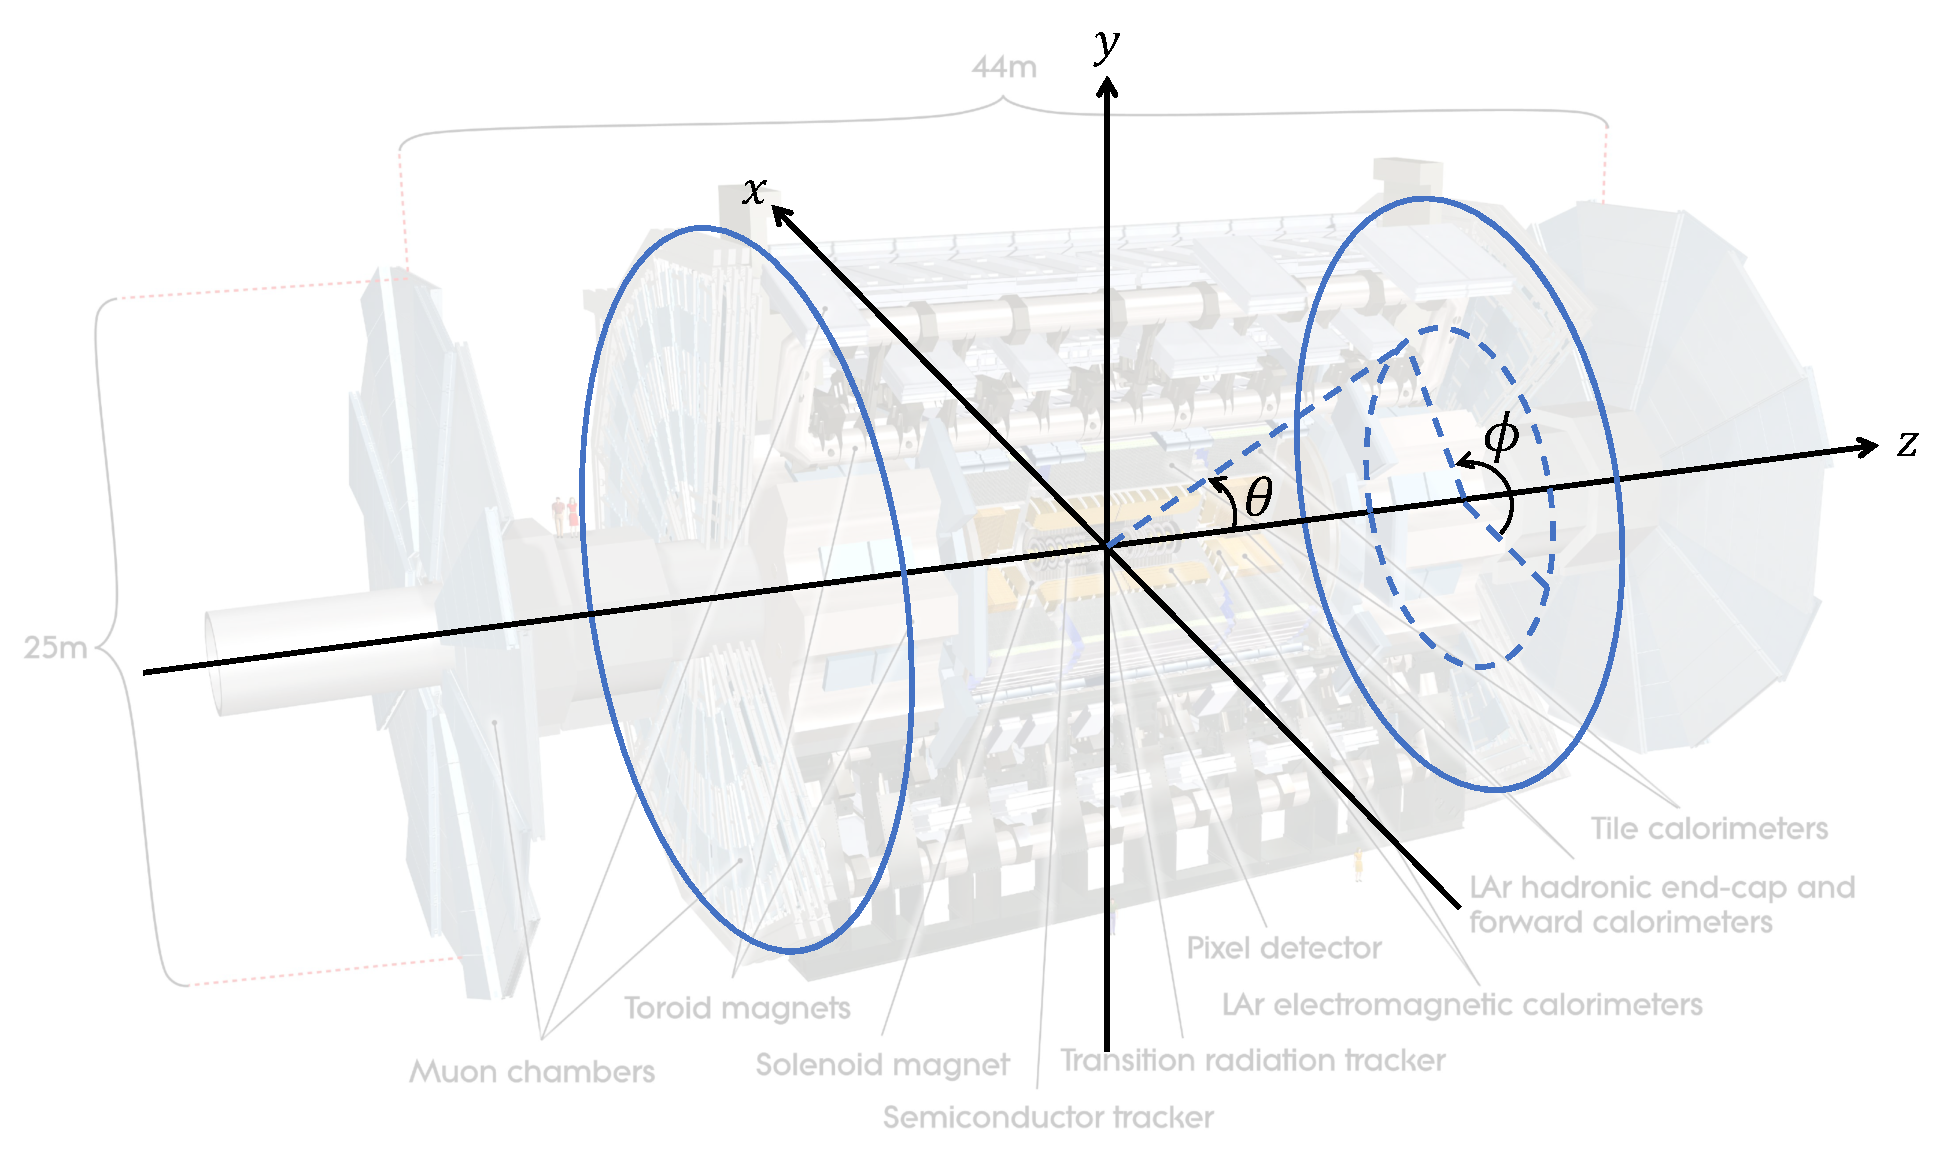
\includegraphics[clip, width=11cm]{fig/2/atlas_coordinate_fix.pdf}
  \caption{ATLAS検出器における座標系。}
  \label{fig:a}
\end{figure}

\newpage
\subsection{マグネットシステム}\label{magnetic_filed}

\subsection{内部飛跡検出器}

\subsection{カロリメータ}

\subsubsection{電磁カロリメータ}

\subsubsection{ハドロンカロリメータ}

\subsection{ミューオン検出器}\label{section2-2-4}

\subsubsection{Resisitive Plate Chamber (RPC)}

\subsubsection{Thin Gap Chambers (TGC)}

\subsubsection{Monitored Drift Tube (MDT)}

\subsubsection{New Small Wheel (NSW)}